\chapter{基于聚类的频率分析攻击方法}
\label{sec:ClusteringAttack}

% The distribution-based attack is based on the assumption that the ordering of ciphertexts in $\mathbf{C}$ reflects that of corresponding plaintexts in $\mathbf{M}$ (recall $\mathbf{M}$ is the original file of $\mathbf{C}$). 

In this section, we relax the adversarial knowledge in the distribution-based attack, and propose the {\em clustering-based attack}, which does not need the fine-grained ordering of plaintexts. Instead, it exploits the {\em similarity} property to infer original data from similar {\em clusters} (i.e., some large data units aggregated by chunks), without relying on the ordering of chunks in each cluster. We first introduce similarity, and then show how to adapt this property into inference attack. 



% In the following, we introduce similarity, followed by how we adapt this property to inference attack.  

\section{Background: Similarity}
\label{sec:similarity}
Similarity \cite{bhagwat09} states that backup files from the same source are likely to be {\em similar} and share a large fraction of identical chunks. The similarity between backup files can be quantified by {\em Broder's theorem} \cite{broder97}. Specifically, if we treat each file as a set $S$ of chunks (i.e., ignore their orders), Broder's theorem states that if the probability that two sets of chunks share the same minimum chunk hash is high, then both sets are likely to share a large fraction of identical chunks and vice versa:  
\begin{eqnarray}
	\Pr[\min\{{\rm H}(S)\} = \min\{{\rm H}(S')\} ] = \frac{|S \cap S'|}{|S \cup S'|}, \nonumber
	\label{eq:broder}
\end{eqnarray}
where ${\rm H}(\cdot)$ is a hash function that is chosen uniformly at random from a min-wise independent family of permutations, and $\min\{{\rm H}(S)\}$ returns the minimum chunk hash of $S$. 
% For easy elaboration, we use {\em MinHash} to denote the minimum element hash of some set. 

Prior works that target different aspects (e.g., performance \cite{qin17,xia11,bhagwat09}, and security \cite{li17}) of deduplication  have applied similarity to {\em preserve storage efficiency}. Specifically, they operate deduplication just on the files that share the same minimum chunk hash (i.e., similar); since similar files can have a large number of identical chunks due to Broder's theorem, such {\em near-exact} deduplication only leads to a slight degradation of storage efficiency. Different from  prior approaches \cite{qin17,xia11,bhagwat09,li17}, we apply similarity to increase the severity of frequency analysis.   


% Thus, prior works   apply chunk-based deduplication across similar segments, so as to improve the effectiveness of {\em near-exact} deduplication. 




% the probability that two sets (files)     
% if two sets share a large fraction of common elements (i.e., they are highly similar), then the probability that both sets share the same minimum hash element is also high.
% likely to be highly similar and share a large fraction of identical chunks. The similarity of  
% The similarity of files can be  Specifically, we treat each file as a set of chunks, and do not care the order of each chunk.   
% that are possibly under different orders yet. Previous approach (e.g., \cite{xia11,bhagwat09}) exploits this property to minimize the memory usage of deduplication.    

% the similarity-based approach that is commonly used to improve deduplication performance \cite{qin17,xia11,bhagwat09}. Then, we show how to adapt the similarity property to inference attack.   


% infer ciphertext-plaintext pairs that are in similar clusters, without the knowledge of the order information of each ciphertext or plaintext in the clusters. 
% consider to relax such ordering leakage. Specifically, we 90  
% We assume that the adversary learns the (generic) order information in a {\em coarse-grained unit}, in which a number of chunks appear together as a set; while the adversary cannot identify the accurate order of any chunk in each set.   


% has some limitations. First, the attack assumes that the adversary has full knowledge of neighboring chunks. Although it is plausible for some deduplicaton systems \cite{xia11,lillibridge09,zhu08}, we can address the assumption by simply swapping the orders of chunks (see \S\ref{sec:countermeasure}). Second, the attack depends on the prevalence of locality in workloads, and it may perform poor in the low-locality workloads. 

% Informed by the limitations (see \S\ref{sec:distribution-discussion}), we consider an attack against the {\em low-locality} workloads, where there does not exist a large stretch of repeated data across backups. We argue that such a workload is reasonable in practice. For example, if multiple users upload their data simultaneously, the chunks received by the server will be disordered and lose locality. 

% Thus, there is no locality among the chunks that arrives in a window of time. 
% continuous data protection (CDP) only stores the chunks where information has changed, it destroys the locality of chunks since changes often appear in unpredictable regions. Thus, for low-locality workloads, the information perceived by the adversary no longer reflect the actual logical orders of chunks.  


% To model the scenario, we consider {\em time window}, which is the basic unit of period whose actual order can be perceived by the adversary. Specifically, we assume that the network bandwidth is steady, and the server can receive a fixed amount (e.g., 4MB) of data during each time window. The adversary cannot distinguish the actual logical orders of chunks that are received within the same time window, while it can learn if two chunks are received in an identical time window. 


% Formally, we use ${\sf tw}(M)$ to denote the orders of the time windows during which the chunk $M$ is received by the server, if we upload all chunks in order. 

% Suppose that all chunks are uploaded under their logical orders. We use ${\sf tw}(M)$ to denote the orders of the time windows during which $M$ is received by the server (note that a chunk may appear multiple times and hence in several time windows). This is the only information about ordering that can be perceived by the adversary. Thus, we can define the leakage:  

% \begin{itemize}[leftmargin=2em]
% 	\item  $\widetilde{\mathcal{L}}_{\rm order} = \{(C, {\sf tw}(M)): M \in \mathbf{M}_{\rm t} \textrm{ and } C = {\sf E}_{K_M}(M)\}$, in which each pair leaks the time window of the original chunk. Note that $\widetilde{\mathcal{L}}_{\rm order}$ no longer implies $\mathcal{L}_{\rm freq}$, since a chunk possibly appears multiple times in the same time window.     
% \end{itemize}



% In this section, we propose a new inference attack, the {\em clustering-based attack}, which can increase the severity of frequency analysis with only the coarse-grained order information like time window, i.e., $\mathcal{L} = (\mathcal{L}_{\rm freq}, \widetilde{\mathcal{L}}_{\rm order})$. 

% does not need the accurate knowledge about neighboring relationships. 

% In this section, we consider the leakage of {\em coarse-grained order information}.  
%    we propose a new inference attack, the {\em clustering-based attack}, which does not need the accurate knowledge about neighboring relationships. Instead, we model $\mathbf{M}_{\rm tar}$ as a collection of {\em chunk regions}, and each region includes a set of continues chunks. The adversary only knows the logical orders of regions, while the orders of chunks in each region are randomly scrambled. 
% Instead, it builds on the  in which the adversary only needs to know the logical order of coarse-grained set of continues chunks, while the orders of chunks in each set are scrambled. More formally, we define the coarse-grained order leakage $\widetilde{\mathcal{L}}_{\rm order}$, ...    
% an obfuscated version of order leakage $\widetilde{\mathcal{L}}_{\rm order}$, based on which the adversary can only know: (i) and (ii) the orders of chunks in each region have been randomized.



% does not need the accurate knowledge about neighboring relationships. Instead, we model $\mathbf{M}_{\rm tar}$ as a collection of {\em chunk regions}, and each region includes a set of continues chunks. The adversary only knows the logical orders of regions, while the orders of chunks in each region are randomly scrambled. 

% A challenge of the attack is how to break ties.

% \subsection{Similarity-based Approaches}
% For example, in a NAS-based backup storage system, the identical chunks are possibly arrived in random order from different clients.  


% coming from different clients are possibly arrived in random order.  
% Since two backups from the same data source are expected to be highly similar and share a large number of identical chunks


% Previous similarity-based approaches \cite{li17,qin17,xia11,bhagwat09} address deduplication performance of such workloads via the Broder's theorem.   
% Previous similarity-based approaches \cite{li17,qin17,xia11,bhagwat09} address the performance bottleneck of deduplication storage systems via Broder's theorem.     
% improves deduplication performance based on :  


% Previous similarity-based approaches 

% In other words, there does not exist   


% in which the chunks are possibly associated with random orders. The stretch of the data, although having the same content, their chunks are associated with random orders.   

% Informed by the limitations (see \S\ref{sec:distribution-discussion}), we consider an attack against the {\em low-locality} workloads, where there does not exist a large stretch of repeated data across backups. We argue that such a workload is reasonable in practice. For example, if multiple users upload their data simultaneously, the chunks received by the server will be disordered and lose locality. 

\section{Description of Clustering-based Attack}
\label{sec:clustering-attack-description}

\begin{figure}
	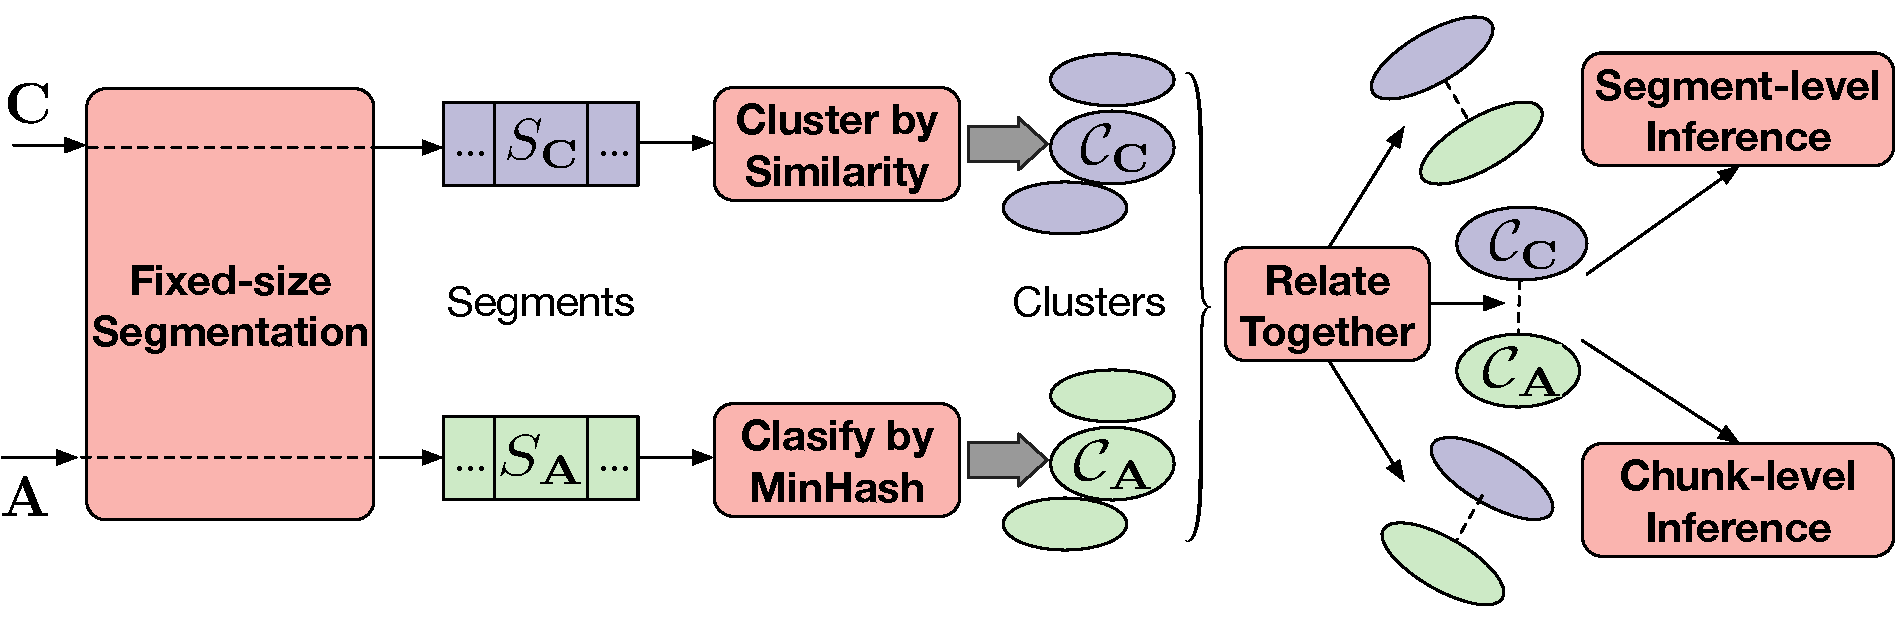
\includegraphics[width=.48\textwidth]{pic/clustering-attack-new.pdf}
    % \caption{Workflow of clustering-based attack: MinHash denotes the minimum chunk hash of plaintext segment, $e(\mathcal{C}_\mathbf{C})$ and $e(\mathcal{C}_\mathbf{A})$ denote the entropies based on the frequency distributions in $\mathcal{C}_\mathbf{C}$ and $\mathcal{C}_\mathbf{A}$, respectively, and  $\#\mathcal{C}_\mathbf{C}$ and $\#\mathcal{C}_\mathbf{A}$ denote the total number of logical ciphertexts and plaintexts in $\mathcal{C}_\mathbf{C}$ and $\mathcal{C}_\mathbf{A}$, respectively.}
    \caption{Workflow of clustering-based attack: MinHash denotes the minimum chunk hash of a plaintext segment.}
	\label{fig:clustering-attack}
\end{figure}

We now present the clustering-based attack (Figure~\ref{fig:clustering-attack}) that builds on similarity to infer original data against encrypted deduplication. 


To exploit similarity, we first introduce {\em segmentation} on a stream of chunks. Specifically, we partition $\mathbf{C}$ into a set of coarse-grained data units, called {\em ciphertext segments}. Each ciphertext segment, denoted by $S_\mathbf{C}$, comprises multiple adjacent ciphertexts in $\mathbf{C}$. In this work, we implement the {\em fixed-size} segmentation scheme to ensure that all ciphertext segments are of the same size (e.g., 4MB by default). 
For compatibility, the same fixed-size segmentation scheme also applies to the auxiliary information $\mathbf{A}$, so as to generate multiple {\em plaintext segments}, each of which is denoted by $S_\mathbf{A}$. 
Note that some variable-size segmentation schemes \cite{lillibridge09, qin17}  identify segment boundaries after the chunks whose contents match a specific pattern and thus address the boundary shift problem faced by the fixed-size segmentation scheme. 
However, we cannot use these variable-size segmentation schemes \cite{lillibridge09, qin17} in the attack. The reason is that the original contents of chunks in ciphertext segments are protected by symmetric encryption, and we cannot ensure that the boundaries for both ciphertext and plaintext segments match the same pattern. This leads to an incompatibility between ciphertext and plaintext segments, and degrades the amount of segment-level data inferred by the clustering-based attack (see the late part of this section).    

% It violates compability, since we cannot   

% It impossible to ensuring the boundaries for  plaintext and ciphertext segments match the same pattern.   

% Even we apply the variable-size segmentation scheme directly  on the contents of ciphertexts, 

% we cannot derive the same pattern for both      



% Note that the order and size of each ciphertext in $\mathbf{C}$ are necessary for operating the fixed-size segmentation, while we do {\em not} need them to reflect those of corresponding plaintext; 


% , so as to be robust against boundary shift of fixed-size segment.  
% we cannot apply
% that match specific content patterns,   
% which address the boundary shift of fixed-size segment, yet requiring to identify segment boundaries that match specific content patterns so as to remain robust against content shifts  
% operate more  requiring the original content patterns of ciphertexts in $\mathbf{C}$. 
 
We propose to infer ciphertext-plaintext pairs through similar segments. Let $S_\mathbf{M}$ be the original plaintext segment of a ciphertext segment $S_\mathbf{C}$ (i.e., each plaintext in $S_\mathbf{M}$ corresponds to some ciphertext in $S_\mathbf{C}$ and vice versa). According to Broder's theorem, if $S_\mathbf{M}$ shares the same minimum chunk hash, say $h$, with some plaintext segment $S_\mathbf{A}$, then $S_\mathbf{M}$  and $S_\mathbf{A}$ tend to have a large fraction of identical plaintexts. This implies that the ciphertexts in $S_\mathbf{C}$ are likely to be mapped from the plaintexts in  $S_\mathbf{A}$. In other words, we first classify all plaintext segments of $\mathbf{A}$ by their minimum chunk hashes, and obtain multiple {\em plaintext clusters}. Each plaintext cluster, denoted by $\mathcal{C}_\mathbf{A} = \{ S_\mathbf{A} \}$, corresponds to a unique minimum chunk hash shared by its included segments. We also 
group the ciphertext segments, whose original plaintext segments have the same minimum chunk hash $h$ (i.e., similar), into an identical {\em ciphertext cluster}, denoted by $\mathcal{C}_\mathbf{C} = \{ S_\mathbf{C} \}$. Then, we infer the original data of $\mathcal{C}_\mathbf{C}$ from some $\mathcal{C}_\mathbf{A}$ that corresponds to  $h$. 

   

% corresponding segment that is mapped to $S_\mathbf{C}$ (i.e., each plaintext in $S_\mathbf{M}$ corresponds to some ciphertext in $S_\mathbf{C}$, and visa versa). 
% Given a ciphertext segment $S_\mathbf{C}$, let 

% if  in other words,  Thus, we propose to launch frequency analysis through similar segments. 
% Specifically,   



% say $\mathcal{C}_\mathbf{C}$.  
% $h$ 
% We denote a plaintext cluster by , which includes multiple  plaintext segments that have the same minimum chunk hash.    
% Each plaintext cluster, denoted by  is a set of  We propose to also collect the ciphertext segments (as a {\em ciphertext cluster} denoted by $\mathcal{C}_\mathbf{C}$) whose original plaintext segments share an identical minimum chunk hash $h$, and then infer their original contents from
% some $\mathcal{C}_\mathbf{A}$ that corresponds to $h$ (i.e., the minimum chunk hash of each plaintext segment in $\mathcal{C}_\mathbf{A}$ equals $h$).    



% and $h$ be the minimum chunk hash computed from $S_\mathbf{M}$.

% Our insight is if $h$ equals the minimum chunk hash of some $S_\mathbf{A}$, then the ciphertexts in $S_\mathbf{C}$  The rationale is the original segment of $S_\mathbf{C}$ has a large fraction of identical plaintexts with $S_\mathbf{A}$ due to Broder's theorem. 



% In other words,   

% This is expected to reduce the disturbances to frequency analysis.  


% $\{S_\mathbf{C}\}$ that have an identical {\em original} minimum element hash $h$,  

% composed of the segments that have the same minimum element hash.  
% However, the original data of each ciphertext segment $S_\mathbf{C}$ is protected by symmetric encryption, and it is impossible to identify the corresponding minimum chunk hash $h$ for grouping ($h$ is derived from the original plaintext segment of $S_\mathbf{C}$). The challenge is how to group similar ciphertext segments {\em without} knowing the minimum chunk hash $h$ of each $S_\mathbf{C}$.    


% the original content of each ciphertext segment $S_\mathbf{C}$ is protected by symmetric encryption; this makes it impossible to identify the corresponding  $h$ for grouping (recall $h$ is derived from the original plaintext segment of $S_\mathbf{C}$). In other words, there exists a challenge of     

We propose a {\em clustering} scheme to group similar ciphertext segments. A na\"{i}ve approach is to classify segments by their minimum chunk hashes, but it does not work on ciphertext segments, whose original contents are protected by symmetric encryption. We address the classification issue based on Broder's theorem.   
% operate classification by the  of each segment , but it .   
Our insight is that if two ciphertext segments have a large fraction of identical ciphertexts, then  they correspond to the same minimum chunk hash with a high probability. The reason is that deterministic encryption preserves the cardinalities of union and intersection of plaintext segments, based on which we can use Broder's theorem to learn the equivalence of their minimum chunk hashes.    
% the fraction of identical plaintexts, based on  Thus, we  apply a clustering algorithm, and aggregate similar ciphertext segments into the same cluster.  

In this work, we define the {\em clustering distance} $d(S_\mathbf{C}, S_\mathbf{C}')$ of any two ciphertext segments $S_\mathbf{C}$ and $S_\mathbf{C}'$ by one minus the fraction of their identical ciphertexts:
\begin{eqnarray}
d(S_\mathbf{C}, S_\mathbf{C}') = 1 - \frac{|S_\mathbf{C} \cap S_\mathbf{C}'|}{|S_\mathbf{C} \cup S_\mathbf{C}'|}. \nonumber
\end{eqnarray}
Note that identical ciphertexts may repeat in $S_\mathbf{C}$ or $S_\mathbf{C}'$, and $|S_\mathbf{C} \cap S_\mathbf{C}'|$ and $|S_\mathbf{C} \cup S_\mathbf{C}'|$ return the number of {\em unique} ciphertexts in their  intersection and union, respectively. Clearly,  the smaller $d(S_\mathbf{C}, S_\mathbf{C}')$ is, the more likely are $S_\mathbf{C}$ and $S_\mathbf{C}'$ to correspond to the same minimum chunk hash. Then, we adopt the {\em agglomerative hierarchical clustering (AHC)} \cite{johnson67} to aggregate similar ciphertext segments based on their distance information.  
Specifically, we start with eash ciphertext segment in its own singleton cluster, and iteratively combine the two closest clusters based on the maximum distance of their ciphertext segments. We configure a parameter $k$, 
% to indicate the upper bound distance in combination, 
and stop the iterated combination when the maximum distance of ciphertext segments in the two cloest
clusters is greater than $k$.


% finally stop combination when       
% Specifically, the clustering scheme is configured by a minimum intercluster distance $d$.   
% We combine nearby segments into clusters based on the distance metric, and stop the combination when 
% the maximum distance between any segment in two clusters is less than $d$.
% the first cluster and any single data point in the second cluster.
% Based on the distance definition, 
% we implement the clustering algorithm via {\em ALGLIB} \cite{alglib}, which is a programming library for extensive data analysis. While ALGLIB supports multiple clustering algorithms, we choose the , because we  only have the distance information of  segments (rather than their coordinates). 
% Specifically, we configure a desired minimum intercluster distance $d$ (e.g., 0.8 by default) via ${\tt clusterizerseparatedbydist()}$, and generate multiple ciphertext clusters via ${\tt clusterizerrunahc()}$.    

For each aggregated ciphertext cluster $\mathcal{C}_\mathbf{C}$, we relate it to some plaintext cluster $\mathcal{C}_\mathbf{A}$ with frequency analysis, while taking frequency distribution into account. This is based on the observation that identical ciphertexts (resp. plaintexts) may  repeat in the same or different ciphertext (resp. plaintext) segments and identical ciphertext (resp. plaintext) segments may also repeat in the same ciphertext (resp. plaintext) cluster. We propose to examine the frequency distribution of the logical ciphertexts or plaintexts in each cluster, and perceive that the frequency distributions for similar clusters (i.e., correspond to the same minimum chunk hash) are also likely to be similar. 
% {\bf Our rationale is changes to backups only apply on limited regions, and do not modify the spatiality of majority chunks.} 

% We proceed the frequency analysis scheme as follows. First, we  sort available ciphertext and plaintext clusters by the total number of logical  ciphertexts and plaintexts they include, respectively. Then, we count the entropy of each cluster based on the frequency distribution of its logical ciphertexts or plaintexts. Like the distribution-based attack (see Section~\ref{sec:distribution-attack-description}), we configure the frequency analysis scheme with the parameters $(u, r, t)$, and infer the ciphertext cluster $\mathcal{C}_\mathbf{C}$ is similar to a plaintext cluster $\mathcal{C}_\mathbf{A}$, if they satisfy the following requirements:    
We proceed the frequency analysis scheme as follows. First, we  sort available ciphertext and plaintext clusters by the total number of logical  ciphertexts and plaintexts they include, respectively. Then, we count an associative array $\mathbf{F}$ that stores the frequency of each unique ciphertext or plaintext in  corresponding cluster. Based on $\mathbf{F}$, we compute the probability that a  ciphertext $C$ exists in a ciphertext cluster $\mathcal{C}_\mathbf{C}$ and further the   
entropy of $\mathcal{C}_\mathbf{C}$:      
% entropy of each ciphertext cluster $\mathcal{C}_\mathbf{C}$:    
\begin{eqnarray*}
    \Pr[C \in \mathcal{C}_\mathbf{C}] = \frac{\mathbf{F}[\mathcal{C}_\mathbf{C}][C]}{\sum_{C' \in \mathcal{C}_\mathbf{C}} \mathbf{F}[\mathcal{C}_\mathbf{C}][C']}, \\
    e(\mathcal{C}_\mathbf{C}) = \sum_{C \in \mathcal{C}_\mathbf{C}} \log_2 \frac{1}{\Pr[C \in \mathcal{C}_\mathbf{C}]},  
    % e(\mathcal{C}_\mathbf{M}) = \sum_{M \in \mathbf{F}[\mathcal{C}_\mathbf{M}]} \log_2 \frac{\mathbf{F}[\mathcal{C}_\mathbf{M}][M]}{a} 
\end{eqnarray*}
where   
$\mathbf{F}[\mathcal{C}_\mathbf{C}][C]$  stores the frequency of $C$ in $\mathcal{C}_\mathbf{C}$. Similarly, we  compute the entropy $e(\mathcal{C}_\mathbf{A})$ for the plaintext cluster $\mathcal{C}_\mathbf{A}$.   
Like the distribution-based attack (see Section~\ref{sec:distribution-attack-description}), we configure the frequency analysis scheme with the parameters $(u, r, t)$, and infer that the ciphertext cluster $\mathcal{C}_\mathbf{C}$ is similar to a plaintext cluster $\mathcal{C}_\mathbf{A}$, if they satisfy the following requirements:
% the entropy of each cluster based on the frequency distribution of its logical ciphertexts or plaintexts. Like the distribution-based attack (see Section~\ref{sec:distribution-attack-description}), we configure the frequency analysis scheme with the parameters $(u, r, t)$, and infer the ciphertext cluster $\mathcal{C}_\mathbf{C}$ is similar to a plaintext cluster $\mathcal{C}_\mathbf{A}$, if they satisfy the following requirements:    
\begin{itemize}[leftmargin=*]
    \item  The rank of $\mathcal{C}_\mathbf{C}$ is not larger than $u$.
    \item  The rank difference of $\mathcal{C}_\mathbf{C}$ and $\mathcal{C}_\mathbf{A}$ is not larger than $r$.  
    \item  The difference of $e(\mathcal{C}_\mathbf{C})$ and $e(\mathcal{C}_\mathbf{A})$ is the smallest and also not larger than $t$.
\end{itemize}

% Thus, the ciphertexts or plaintexts in each cluster may follow a non-uniform frequency distribution, and such frequency distributions are further correlated for the similar clusters  in different backups.  
% We expect  ciphertexts or plaintexts in most of clusters follow a non-uniform frequency distribution, and such frequency distributions are {\em correlated} for  similar clusters (i.e., correspond to the same minimum chunk hash) in different backups. 
% Our rationale is .   
% Thus, we apply a  scheme like the distribution-based frequency analysis (see Section~\ref{sec:distribution-attack-description}), in order to find similar clusters. 

Then, for each pair $(\mathcal{C}_\mathbf{C}, \mathcal{C}_\mathbf{A})$ of similar clusters, we infer ciphertext-plaintext pairs in two levels. 
\begin{itemize}[leftmargin=*]
    \item {\bf Segment-level inference:}
        If $\mathcal{C}_\mathbf{C}$ and $\mathcal{C}_\mathbf{A}$ have the same number of logical chunks (i.e., ciphertexts or plaintexts), as well as an identical entropy, this implies that $\mathcal{C}_\mathbf{C}$ is exactly mapped from $\mathcal{C}_\mathbf{A}$ with a high probability. In this case, we operate attack on the coarse-grained {\em segment} level. Specifically, we first compute the entropies of each ciphertext segment $S_\mathbf{C}$ in $\mathcal{C}_\mathbf{C}$ and each plaintext segment $S_\mathbf{A}$ in $\mathcal{C}_\mathbf{A}$, based on the frequency distributions of their ciphertexts and plaintexts, respectively. 
        % (recall identical chunks may have duplicate copies in the same segment). 
         We infer that $S_\mathbf{C}$ is mapped from  $S_\mathbf{A}$, if the total numbers of logical chunks, as well as the entropies, of $S_\mathbf{C}$ and $S_\mathbf{A}$ are identical. Our evaluation shows that the segment-level inference contributes most of the correctly inferred contents in the
        clustering-based attack (see
        Section~\ref{sec:experiment-clustering}). It is also possible to further recover each plaintext in these inferred segments with additional adversarial knowledge (e.g., ordering). 

        
    \item {\bf Chunk-level inference:}
        If $\mathcal{C}_\mathbf{C}$ and $\mathcal{C}_\mathbf{A}$ have different numbers of logical chunks or entropies, we apply frequency analysis to operate attack on the fine-grained {\em chunk} level. Specifically, we sort all unique ciphertexts and plaintexts by their frequencies in $\mathcal{C}_\mathbf{C}$ and $\mathcal{C}_\mathbf{A}$, respectively, and infer ciphertext-plaintext pairs based on frequency ranks.  
        However, we find the chunk-level inference does not perform well in our experimental dataset. The possible reason is each cluster includes a large number of logical chunks, which degrades the effectiveness of  frequency analysis. Even so, we expect the chunk-level inference can recover more ciphertext-plaintext pairs in practice, especially when the number of logical chunks in some clusters is limited.   
        % there are many tied chunks in the similar classes of the VM dataset
        % Even so, we still expect it can recover even more information in practice, especially when each cluster is of .  
\end{itemize}

% Figure~\ref{fig:clustering-attack} puts all design primitives together, and show the workflow of the clustering-based attack.


\subsection{Summary:}
To summarize, the clustering-based attack exploits similarity, and launches frequency analysis in similar clusters to infer ciphertext-plaintext pairs. In addition to  $u$, $r$ and $t$, it is configured by the parameter $k$, which specifies the upper bound distance in combining the closest clusters.   

Although possibly affected by the boundary shift of fixed-size segments, we argue that the clustering-based attack is severe against VM disk images. 
Specifically, a flat VM image file is allocated of a fixed size at the time it is created, and such size cannot be changed during its lifetime. All unused regions in a VM image are initially filled with  zero chunks, which can be further re-written for storing additional data in the image. 
% The clustering-based attack does not suffer from boundary shift in this case, since VM images do not need to insert or remove chunks. 
In Section \ref{sec:experiment-clustering}, we examine the effectiveness of the clustering-based attack against VM images.

% One limitation of the clustering-based attack is it suffers from the {\em boundary shift} of segment. Specifically, since we apply fixed-size segmentation, the insertion of one or more chunks will shift the boundaries of all segments that come after the insertion point. This changes the frequency distribution of chunks in some segments, and affects the precision of the identified similar clusters. This also leads to a reduced number of identical segments, and degrades the amount of original contents inferred by the segment-level inference. 
% % Our evaluation shows that the clustering-based attack can only infer about 1\% original content in a long-term backup dataset. 
% We argue that the clustering-based attack is still severe for {\em VM disk images}.    
     

% After allocation, all unused regions in the image are filled by , and   
% which of {\em fixed} sizes during their lifetime.  
% . Specifically, a flat image file is allocated of a {\em fixed} size at the time it is created, and all unused regions of the image file are initially filled with {\em zero chunks}. The image file can store additional data by re-writing zero chunks   
%  Flat images are fixed-size files, with one block for each block in the guest’s disk. Initially, unused blocks are zero-filled; thus, flat disk images tend to have a lot of zero-filled blocks, particularly if they are rela- tively large to allow the guest operating system space into which to store additional data. Sparse images, unlike flat im- ages, only contain virtual disk blocks that have been written at least once. Thus, sparse images can occupy relatively lit- tle space when created, and only grow as the guest operating system uses more and more of its virtual disk. Note, how- ever, that sparse images can
% contain zero-filled blocks, since the guest operating system may write a block containing all zeros; such a block would be stored by the virtual machine in the disk image file. While there is no global standard for virtual machine disk images, specifications for one file format is available from VMware 

% the clustering-based attack has low effectiveness (about 1% inference rate) against the FSL dataset.

% Even so, we argue that the clustering-based attack is severe for some workloads, which store data {\em aligned} with disk block boundaries and do not have the problem of  \cite{jin09}. In \S\ref{sec:experiment-clustering}, we will examine the effectiveness of the clustering-based attack against VM workloads,   



% The main limitation of the clustering-based attack is the {\em boundary shift} of segment.  This changes the chunk distributions of some segments, and  affects the precision of identifying similar classes in Step 2. The boundary shift also decreases the effectiveness of the segment-level attack in Step 3, since it leads to fewer common segments in the auxiliary data and target data. On the other hand, we cannot address the boundary-shift problem by existing approaches (e.g., the content-defined segmentation \cite{lillibridge09}), which depend on the knowledge of the underlying content pattern of ciphertext chunks. 



%% In \S\ref{sec:clustering-experiment}, we justify the barrier of the boundary shift in the clustering-based attack.       
% % between $\mathbf{M}_{\rm a}$ and $\mathbf{M}_{\rm t}$,  
%%We adapt the similarity-based approach to inference attack. Specifically, we apply segmentation, yet on ciphertext chunks, and generate the segments that include adjacent ciphertext chunks under the scrambled order in $\widetilde{\mathcal{L}}_{\rm order}$. 



%If $\mathcal{C}_i$ and $\mathcal{M}_j$ have different numbers of logical chunks or entropies, we apply operate classical frequency analysis to operate attack on {\em chunk level}. This can infer more ciphertext-plaintext chunk pairs, yet degrading inference precision.

%% over $\mathcal{C}_i$ and $\mathcal{M}_j$ . 
%% for each ciphertext segment in $\mathcal{C}_i$, we find the plaintext segment that has the same  
%% Specifically, for each ciphertext segment $S_{\rm t}$ in $\mathcal{C}_i$, we find the plaintext segment $S_{\rm a}$ in $\mathcal{S}_j$ such that   
%% Then, we adopt the idea of distribution-based ranking (\S\ref{sec:distribution-attack-description}) to identify the ciphertext and plaintext classes that are identified by the same MinHash.  
%%In the following, we first propose the {\em similarity-based clustering} approach, which aims to classify ciphertext segments by their underlying MinHash. Then, we elaborate how to relate a class of ciphertext segments with that of plaintext segments. 
%%\paragraph{Similarity-based clustering:}
%%works on ciphertext segments and classify them by their underlying MinHash. Then,   



% \paragraph{Step 3: (Launch attack through similar classes):} For each identified similar classes $(\mathcal{C}_i, \mathcal{M}_j)$, we launch attack for two cases. If $\mathcal{C}_i$ and $\mathcal{M}_j$ have the same number of logical chunks and entropy, our attack operates on {\em segment level}. For each ciphertext segment $S_{\rm t}$ in $\mathcal{C}_i$, we examine each available plaintext segment $S_{\rm a}$ in $\mathcal{S}_j$, and infer $(S_{\rm t}, S_{\rm a})$ as a ciphertext-plaintext segment pair if $S_{\rm a}$ has the same number of logical chunks and entropy (via Equation~\ref{eq:clustering-entropy} but computed for segment) with $S_{\rm t}$. We stop the attack at segment level in this case, because there is not enough information to further extracting chunk content; otherwise it sacrifices inference precision. We argue that the segment-level attack is severe, since each segment represents a continues region of data. The adversary can learn significant information if it successfully extracts the underlying data of some segment. 

%% Through experimental analysis, the segment-level attack contributes the most component of correct inferences.     
%% has the same number of logical chunks and entropy as $S_{\rm t}$. We infer that $S_{\rm a}$ is the original segment of $S_{\rm t}$. 

%If $\mathcal{C}_i$ and $\mathcal{M}_j$ have different numbers of logical chunks or entropies, we apply operate classical frequency analysis to operate attack on {\em chunk level}. This can infer more ciphertext-plaintext chunk pairs, yet degrading inference precision.

%% over $\mathcal{C}_i$ and $\mathcal{M}_j$ . 
%% for each ciphertext segment in $\mathcal{C}_i$, we find the plaintext segment that has the same  
%% Specifically, for each ciphertext segment $S_{\rm t}$ in $\mathcal{C}_i$, we find the plaintext segment $S_{\rm a}$ in $\mathcal{S}_j$ such that   
%% Then, we adopt the idea of distribution-based ranking (\S\ref{sec:distribution-attack-description}) to identify the ciphertext and plaintext classes that are identified by the same MinHash.  
%%In the following, we first propose the {\em similarity-based clustering} approach, which aims to classify ciphertext segments by their underlying MinHash. Then, we elaborate how to relate a class of ciphertext segments with that of plaintext segments. 
%%\paragraph{Similarity-based clustering:}
%%works on ciphertext segments and classify them by their underlying MinHash. Then,   



% Based on the configuration parameters of $u$, $r$ and $t$ (see \S\ref{sec:distribution-attack-description}), we pick the ciphertext class $\mathcal{C}_i$ that has the $i$-th most number of logical chunks ($1 \leq i \leq u$), and examine each plaintext class $\mathcal{M}_j$ that ranks from $i-r$ to $i+r$. We identify that $\mathcal{C}_i$ and $\mathcal{M}_j$ have the same MinHash, if the difference of their entropies is (i) minimum across all $i-r \leq j \leq i+r$ and (ii) smaller than $t$.   

   

% while the rest data preserve the same characteristics.   
% Due to backup redundancies, .   . 
% Our rationale is that the chunk distributions in similar classes are likely to be correlated due to deterministic encryption.

%We build on the idea of the distribution-based ranking (see \S\ref{sec:distribution-attack-description}) to identify the ciphertext and plaintext classes that correspond to the same MinHash. Specifically, for each ciphertext class with an underlying MinHash of $h$, our aim is to find the plaintext class identified by the same MinHash of $h$. Note that we cannot measure relative frequency distributions for ranking, since we do not have enough knowledge about neighboring chunks. Instead, we count the entropy of a class by the {\em occurrences of different chunks} in the class. Specifically, for a plaintext class $\mathcal{M}$, we compute its entropy:  \begin{eqnarray}
%        e_{\mathcal{M}} = \sum_{M \in \mathcal{M}} {\sf log}_2 \frac{{\sf cnt}_\mathcal{M}(M)}{|\mathcal{M}|},
%        \label{eq:clustering-entropy}
%\end{eqnarray}
%where $|\mathcal{M}|$ is the total number of logical chunks in $\mathcal{M}$ and ${\sf cnt}_\mathcal{M}(M)$ returns the number of copies of the chunk $M$ in $\mathcal{M}$. We derive similar entropy $e_\mathcal{C}$ for a ciphertext class $\mathcal{C}$, and consider $\mathcal{M}$ and $\mathcal{C}$ are {\em similar classes} (i.e., having the same MinHash), if the difference of their entropies is minimum. Our rationale is that the chunk distributions in similar classes are likely to be correlated due to deterministic encryption.  

%In more details, we first sort the available ciphertext and plaintext classes separately by the number of logical chunks they include. Based on the configuration parameters of $u$, $r$ and $t$ (see \S\ref{sec:distribution-attack-description}), we pick the ciphertext class $\mathcal{C}_i$ that has the $i$-th most number of logical chunks ($1 \leq i \leq u$), and examine each plaintext class $\mathcal{M}_j$ that ranks from $i-r$ to $i+r$. We identify that $\mathcal{C}_i$ and $\mathcal{M}_j$ have the same MinHash, if the difference of their entropies is (i) minimum across all $i-r \leq j \leq i+r$ and (ii) smaller than $t$.   

%% However, it is hard to classify ciphertext segments, since there still exists a challenge on identifying the underlying MinHash of ciphertext segments. Recall that  
%% By our assumption (\S\ref{sec:clustering-attack}), all ciphertext segments must have the same size. Thus, to be compatible, we also partition the original stream of plaintext chunks $\mathbf{M}_{\rm a}$ into fixed-size {\em plaintext segments}, each of which comprises a sequence of plaintext chunks.

%% We adapt the similarity-based approach to inference attack. Specifically, to capture the notion of similarity,  
%% for inferring ciphertext-plaintext chunk pairs through similar segments. Specifically, we   



% We proceed our similarity-based clustering scheme as follows. It defines the {\em clustering distance} of The smaller the distance ${\sf Dist}(S_{\rm t}, S_{\rm t}')$ is, the more likely are $S_{\rm t}$ and $S_{\rm t}'$ to have the same underlying MinHash. Then, it uses the agglomerative hierarchical clustering algorithm (via the function  in ) for clustering, and generates the ciphertext classes based on a desired minimum intercluster distance of $d$ (via the function  in ALGLIB \cite{alglib}). By default, we configure $d$ by 0.8. 



% we can apply Broder's theorem  on ciphertexts due to the deterministic nature of encryption.  
% This is because encryption preserves the deduplication capability of elements.
% . Thus, we can compute the overlaps between any two ciphertext segments, and cluster them into several {\em ciphertext classes}, such that each cluster includes the ciphertext segments that possibly have the same underlying MinHash.    

 


%We propose the {\em similarity-based clustering} approach, which aims to classify the ciphertext segments by their underlying MinHash while not compromising confidentiality. The key insight is that if two ciphertext segments have a large fraction of common (ciphertext) chunks, then they are likely to have the same underlying MinHash (due to Equation (\ref{eq:broder})). Thus, we can compute the overlaps between any two ciphertext segments, and cluster them into several {\em ciphertext classes}, such that each cluster includes the ciphertext segments that possibly have the same underlying MinHash.    




% identify  This raises a challenge on how to group   
% the minimum element hash $h$  
% it is impossible to the original plaintext and identify the minimum element hash corresponding to a ciphertext segment.  
% recover its original plaintext segment and extract the minimum element hash.    
% the original plaintexts of the ciphertext segment, and further learn the      
% The challenge is  Since each ciphertext segment is mapped by symmetric encryption, it is impossible to learn their original content and identify the minimum element hash from corresponding plaintexts.
% Since each ciphertext in $S_\mathbf{C}$ is mapped by symmetric encryption, it is impossible to learn their original plaintexts or identify the minimum element hash (based on these plaintexts). In other words, the main challenge  
% which chunk leads to the minimum element hash, and further the exact hash value. In other words, there exists a challenge on collecting similar $\{ S_\mathbf{C} \}$ (i.e., they share the same original minimum element hash) and map them to $\mathcal{C}_\mathbf{A}$. 


%Thus, instead of inferring ciphertext-plaintext pairs (from $\mathbf{C}$ and $\mathbf{A}$) directly,     


%One challenge behind the clustering-based attack is how to identify the original minimum element hash $h$ of each $S_\mathbf{C}$. Since       


%The clustering-based attack proceeds as follows. First, we  


%We classify plaintext segments into a set of {\em plaintext classes} by their MinHash. On the other hand, we cannot perform similar classification over ciphertext segments, since their underlying contents are protected by symmetric encryption (see \S\ref{sec:threat}). 

%% , each of which includes the plaintext segments that have the same MinHash. 
%% it is impossible to access or compare the underlying contents of ciphertext chunks for classification, since their original contents are protected by symmetric encryption   


%% split the original space () of frequency analysis into multiple subspaces, and
%% eliminates     
%% identify the minimum element hash of each $S_\mathbf{C}$, and then apply frequency analysis with some $S_\mathbf{A}$ that shares the same minimum element hash. This      
%% This inspires us to    
% % $S_\mathbf{M}$ has a large fraction of overlaps with the original plaintexts of $S_{\rm t}$    
%% Our insight is  if the {\em underlying MinHash} (that is computed from the plaintext of each ciphertext chunk element) of a ciphertext segment $S_{\rm t}$ is identified the same as that of some plaintext segment $S_{\rm a}$, then the chunks in $S_{\rm a}$ are likely to be the original plaintexts of the ciphertexts in $S_{\rm t}$. The rationale is that $S_{\rm a}$ has a large fraction of overlaps with the original plaintexts of $S_{\rm t}$  (due to Equation~(\ref{eq:broder})). In other words, we collect all ciphertext segments that have a common underlying MinHash (see Step 1), say $h$, and infer their original chunks from the plaintext segments that have the same MinHash of $h$ (see Step 2 and Step 3). By repeating the inference for each available MinHash, we can avoid some of ties incurred by classical frequency analysis, since the tied chunks may have different frequencies for the same MinHash.    
%% Similarly, we apply fixed-size segmentation to generate each segment $S_\mathbf{A}$ that consists of plaintexts of $\mathbf{A}$.
%% knowledge of the underlying content pattern of ciphertext chunks. 
%% that we need the order of each ciphertext in $\mathbf{C}$ for segmentation, while not requiring such order reflects that of corresponding plaintext. 
%% We use  and  that is generated from $\mathbf{C}$ and that is mapped from, respectively.
%% generated from $\mathbf{C}$ and its corresponding plaintext, respectively.
%% denote a segment from $\mathbf{C}$ by  
%% Note that we need the ordering of $\mathbf{C}$ to ensure each segment includes the continue content, while not requiring such ordering reflects that of corresponding plaintext.  
%% {\em fixed-size} data units,   
%%In this work, we implement fixed-size segmentation scheme to generate ciphertext segments. More sophisticated segmentation schemes (e.g., variable-size segmentation \cite{lillibridge09, qin17}) can be applied to address content shifting, yet they depend on the knowledge of the underlying content pattern of ciphertext chunks. For clustering, we define the distance of two ciphertext segments $S_{\rm tar}$ and $S_{\rm tar}'$ by one minus their Jaccard similarity coefficient:
%%
%% Given $\mathbf{C}$, we partition   
%% The clustering-based attack builds on {\em similarity-based approach} \cite{li17,qin17,xia11,bhagwat09}. Specifically, the similarity-based approach groups multiple adjacent chunks into a coarse-grained unit called {\em segment}, and considers that two segments are {\em similar} if they have the same minimum hash value (i.e., {\em MinHash}) over their chunk elements. By Broder's theorem \cite{broder97}, the probability that two segments $S$ and $S'$ are similar is the same as their Jaccard similarity coefficient: 
%% \subsection{Attack Description}
%% {\color{blue}
%% {\bf --- not good enough ---}
%% To capture similarity in inference attack, we partition the auxiliary stream $\mathbf{M}_{\rm a}$ of plaintext chunks into {\em plaintext segments}, which comprises sequences of plaintext chunks. Correspondingly, we construct {\em ciphertext segments}, each of which is composed of the ciphertext chunks whose original plaintexts are in the same plaintext segment. For compatibility, we ensure that both  plaintext and ciphertext segments have the same size.   
%% {\bf --- not good enough ---}
%% }
%% (recall that we can access the time windows of original chunks from $\widetilde{\mathcal{L}}_{\rm order}$). 
%% We propose to launch inference attack through similar segments. 


%\begin{figure}
%	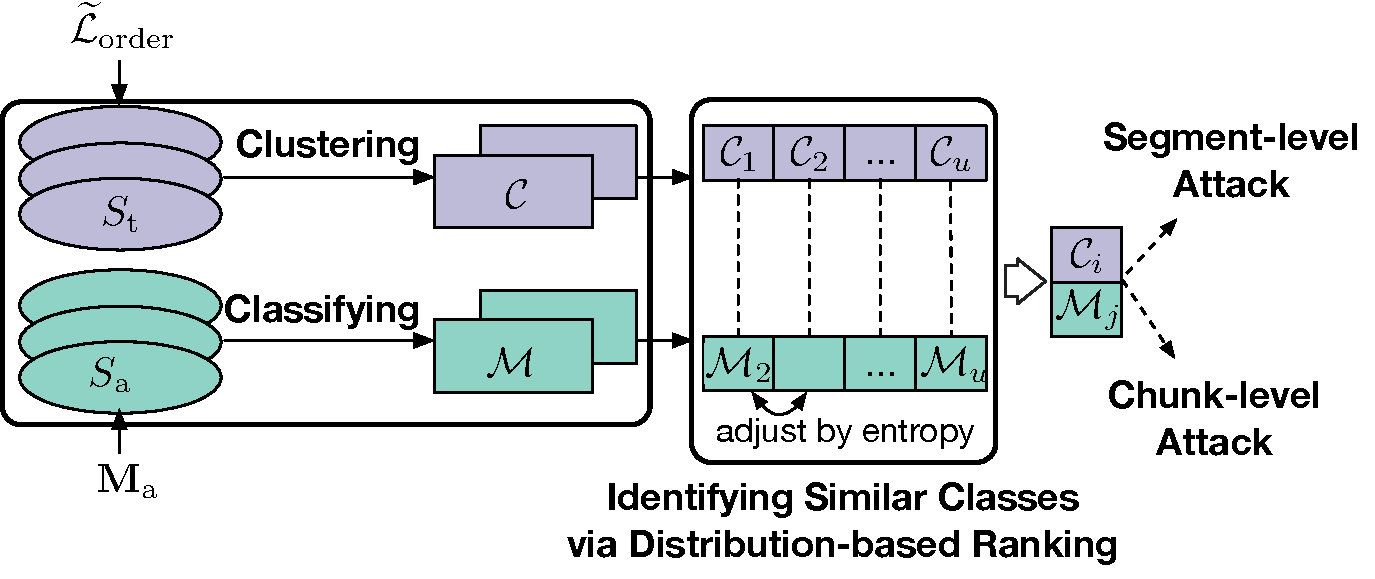
\includegraphics[width=.48\textwidth]{pic/clustering-attack.pdf}
%	\caption{Overview of the clustering-based attack.}
%	\label{fig:clustering-attack}
%\end{figure}

%Figure~\ref{fig:clustering-attack} highlights the main steps of the clustering-based attack. We elaborate the details as follows. 


%\paragraph{Step 2: (Identify similar classes):}
%We build on the idea of the distribution-based ranking (see \S\ref{sec:distribution-attack-description}) to identify the ciphertext and plaintext classes that correspond to the same MinHash. Specifically, for each ciphertext class with an underlying MinHash of $h$, our aim is to find the plaintext class identified by the same MinHash of $h$. Note that we cannot measure relative frequency distributions for ranking, since we do not have enough knowledge about neighboring chunks. Instead, we count the entropy of a class by the {\em occurrences of different chunks} in the class. Specifically, for a plaintext class $\mathcal{M}$, we compute its entropy:  \begin{eqnarray}
%        e_{\mathcal{M}} = \sum_{M \in \mathcal{M}} {\sf log}_2 \frac{{\sf cnt}_\mathcal{M}(M)}{|\mathcal{M}|},
%        \label{eq:clustering-entropy}
%\end{eqnarray}
%where $|\mathcal{M}|$ is the total number of logical chunks in $\mathcal{M}$ and ${\sf cnt}_\mathcal{M}(M)$ returns the number of copies of the chunk $M$ in $\mathcal{M}$. We derive similar entropy $e_\mathcal{C}$ for a ciphertext class $\mathcal{C}$, and consider $\mathcal{M}$ and $\mathcal{C}$ are {\em similar classes} (i.e., having the same MinHash), if the difference of their entropies is minimum. Our rationale is that the chunk distributions in similar classes are likely to be correlated due to deterministic encryption.  


%In more details, we first sort the available ciphertext and plaintext classes separately by the number of logical chunks they include. Based on the configuration parameters of $u$, $r$ and $t$ (see \S\ref{sec:distribution-attack-description}), we pick the ciphertext class $\mathcal{C}_i$ that has the $i$-th most number of logical chunks ($1 \leq i \leq u$), and examine each plaintext class $\mathcal{M}_j$ that ranks from $i-r$ to $i+r$. We identify that $\mathcal{C}_i$ and $\mathcal{M}_j$ have the same MinHash, if the difference of their entropies is (i) minimum across all $i-r \leq j \leq i+r$ and (ii) smaller than $t$.   

%% However, it is hard to classify ciphertext segments, since there still exists a challenge on identifying the underlying MinHash of ciphertext segments. Recall that  
%% By our assumption (\S\ref{sec:clustering-attack}), all ciphertext segments must have the same size. Thus, to be compatible, we also partition the original stream of plaintext chunks $\mathbf{M}_{\rm a}$ into fixed-size {\em plaintext segments}, each of which comprises a sequence of plaintext chunks.

%% We adapt the similarity-based approach to inference attack. Specifically, to capture the notion of similarity,  
%% for inferring ciphertext-plaintext chunk pairs through similar segments. Specifically, we   


%\paragraph{Step 3: (Launch attack through similar classes):} For each identified similar classes $(\mathcal{C}_i, \mathcal{M}_j)$, we launch attack for two cases. If $\mathcal{C}_i$ and $\mathcal{M}_j$ have the same number of logical chunks and entropy, our attack operates on {\em segment level}. For each ciphertext segment $S_{\rm t}$ in $\mathcal{C}_i$, we examine each available plaintext segment $S_{\rm a}$ in $\mathcal{S}_j$, and infer $(S_{\rm t}, S_{\rm a})$ as a ciphertext-plaintext segment pair if $S_{\rm a}$ has the same number of logical chunks and entropy (via Equation~\ref{eq:clustering-entropy} but computed for segment) with $S_{\rm t}$. We stop the attack at segment level in this case, because there is not enough information to further extracting chunk content; otherwise it sacrifices inference precision. We argue that the segment-level attack is severe, since each segment represents a continues region of data. The adversary can learn significant information if it successfully extracts the underlying data of some segment. 


%% Through experimental analysis, the segment-level attack contributes the most component of correct inferences.     
%% has the same number of logical chunks and entropy as $S_{\rm t}$. We infer that $S_{\rm a}$ is the original segment of $S_{\rm t}$. 

%If $\mathcal{C}_i$ and $\mathcal{M}_j$ have different numbers of logical chunks or entropies, we apply operate classical frequency analysis to operate attack on {\em chunk level}. This can infer more ciphertext-plaintext chunk pairs, yet degrading inference precision.

%% over $\mathcal{C}_i$ and $\mathcal{M}_j$ . 
%% for each ciphertext segment in $\mathcal{C}_i$, we find the plaintext segment that has the same  
%% Specifically, for each ciphertext segment $S_{\rm t}$ in $\mathcal{C}_i$, we find the plaintext segment $S_{\rm a}$ in $\mathcal{S}_j$ such that   
%% Then, we adopt the idea of distribution-based ranking (\S\ref{sec:distribution-attack-description}) to identify the ciphertext and plaintext classes that are identified by the same MinHash.  
%%In the following, we first propose the {\em similarity-based clustering} approach, which aims to classify ciphertext segments by their underlying MinHash. Then, we elaborate how to relate a class of ciphertext segments with that of plaintext segments. 
%%\paragraph{Similarity-based clustering:}
%%works on ciphertext segments and classify them by their underlying MinHash. Then,   

%\subsection{Discussion}
%\label{sec:clustering-attack-discussion}

%The main limitation of the clustering-based attack is the {\em boundary shift} of segment. The insertion of one or more chunks will shift the boundaries of all segments that come after the insertion point. This changes the chunk distributions of some segments, and  affects the precision of identifying similar classes in Step 2. The boundary shift also decreases the effectiveness of the segment-level attack in Step 3, since it leads to fewer common segments in the auxiliary data and target data. On the other hand, we cannot address the boundary-shift problem by existing approaches (e.g., the content-defined segmentation \cite{lillibridge09}), which depend on the knowledge of the underlying content pattern of ciphertext chunks. 


%Even so, we argue that the clustering-based attack is severe for the virtual machine (VM) images, which store data {\em aligned} with disk block boundaries  \cite{jin09}. In \S\ref{sec:experiment-clustering}, we will examine the effectiveness of the clustering-based attack against VM workloads. 



%% In \S\ref{sec:clustering-experiment}, we justify the barrier of the boundary shift in the clustering-based attack.       
% % between $\mathbf{M}_{\rm a}$ and $\mathbf{M}_{\rm t}$,  
%%We adapt the similarity-based approach to inference attack. Specifically, we apply segmentation, yet on ciphertext chunks, and generate the segments that include adjacent ciphertext chunks under the scrambled order in $\widetilde{\mathcal{L}}_{\rm order}$. 


%%In this work, we implement fixed-size segmentation scheme to generate ciphertext segments. More sophisticated segmentation schemes (e.g., variable-size segmentation \cite{lillibridge09, qin17}) can be applied to address content shifting, yet they depend on the knowledge of the underlying content pattern of ciphertext chunks. For clustering, we define the distance of two ciphertext segments $S_{\rm tar}$ and $S_{\rm tar}'$ by one minus their Jaccard similarity coefficient:
%%$${\sf Sim}(S_{\rm tar}, S_{\rm tar}') = 1 - \frac{|S_{\rm tar} \cap S_{\rm tar}'|}{|S_{\rm tar} \cup S_{\rm tar}'|}.$$
%%The smaller ${\sf Sim}(S_{\rm tar}, S_{\rm tar}')$ is, the more likely that they have the same underlying MinHash. Then, we use agglomerative hierarchical clustering algorithm (via the function {\tt clusterizerrunahc} in ALGLIB \cite{alglib}) to generate the slices. 

%%% For any two ciphertext segments $S_{\rm tar}$ and $S_{\rm tar}'$, we define their similarity distance by one minus their Jaccard similarity coefficient:
%%% $${\sf Sim}(S_{\rm tar}, S_{\rm tar}') = 1 - \frac{|S_{\rm tar} \cap S_{\rm tar}'|}{|S_{\rm tar} \cup S_{\rm tar}'|}.$$

%%In addition, we partition $\mathbf{M}_{\rm aux}$ to form plaintext segments, each of which is a region of logically adjacent chunks in $\mathbf{M}_{\rm aux}$. For compatibility, we require that the plaintext segment has the same (fixed) size with ciphertext segment. Then, we classify plaintext segments by their MinHash (note that we have full access to the MinHash of each plaintext segment), and obtain several plaintext slices. 

%%To launch attack, we apply frequency analysis to the ciphertext and plaintext slices that are identified by the same MinHash. This is for two reasons. First, tied chunks may have different frequencies in some slices, and these ties can be break. Second, the original chunks are likely to be in the 

%%each of which includes the segments that have the same MinHash (note that we have fully access to the MinHash of each plaintext segment).   



%%Like prior works \cite{li17,qin17,xia11,bhagwat09}, we   




%%Specifically, we  We also generate ciphertext segments, which include adjacent ciphertext chunks yet under the scrambled order in $\widetilde{\mathcal{L}}_{\rm order}$. 



%%The clustering-based attack uses {\em ``divide-and-conquer''} strategy to improve the inference accuracy of tied chunks. At a high level, it partitions $\mathbf{M}_{\rm aux}$ into {\em plaintext slices}, and each slice includes a number of plaintext chunks. It generates similar {\em ciphertext slices} from $\widetilde{\mathcal{L}}_{\rm order}$, and pairs each ciphertext slice with some plaintext slice of $\mathbf{M}_{\rm aux}$. It finally applies frequency analysis to infer original chunks from each slice pair. The rationale is that tied chunks may have different frequencies in some slices.

%%% To generate slices, we build on the {\em similarity-based approach} \cite{li17,qin17,xia11,bhagwat09}. Specifically, it defines a coarse-grained unit called {\em segment}, which comprises multiple adjacent chunks. Two segments are said {\em similar}, if they have the same minimum hash (i.e., MinHash) over their chunk elements. By Broder's theorem \cite{broder97}, the probability that two segments $S_i, S_j$ are similar is the same as their Jaccard similarity coefficient: 
%%% $${\sf Pr}[{\sf MinHash}(S_i) = {\sf MinHash}(S_j)] = \frac{|S_i \cap S_j|}{|S_i \cup S_j|},$$
%%% where ${\sf MinHash}(S)$ is the minimum hash of chunk element in $S$. Thus, prior works \cite{li17,qin17,xia11,bhagwat09} can apply the similarity-based approach to improve the effectiveness of near-exact deduplication. 


%%To form a plaintext slice, we collect all     


%%===


%%Specifically, we add the segments that have the same MinHash into an identical slice, and pair a ciphertext slice with a plaintext slice if they have the same chunk. Thus,  

%%each slice includes the segments that have the same MinHash. Since 

%%the original chunk of ciphertext chunk is likely to be in  


%%Our insight is that if two ciphertext segments have a large fraction of common chunks, they are likely to have the same underlying MinHash.


%%By Broder's theorem, similar segments are likely to have a large fraction of common chunks.  


%%Our insight is to generate slices  



%%A plaintext segment is a region of logically adjacent chunks in $\mathbf{M}_{\rm aux}$, while a ciphertext segment includes several adjacent ciphertext chunks defined in the scrambled order in $\widetilde{\mathcal{L}}_{\rm order}$. We measure the {\em similarity} of two segments (e.g., $S_i$ and $S_j$) by their Jaccard similarity coefficient (e.g., $|S_i \cap S_j|/|S_i \cup S_j|$).     

%%Our insight is to generate the slices that include all segments identified by the same MinHash.  



%%We propose a new inference attack, the {\em clustering-based attack}, which uses {\em ``divide-and-conquer''} strategy to improve the severity of frequency analysis.   
   

%%The clustering-based attack builds on  




%%The key technique underlying the attack is {\em similarity-based approach} to generate slices.  

%%To generate slices, the clustering-based attack uses a {\em similarity-based approach}, which builds on a coarse-grained unit, called {\em segment}, of chunks. A plaintext segment is a region of logically adjacent chunks in $\mathbf{M}_{\rm aux}$. We also extract ciphertext segments, which include adjacent ciphertext chunks defined in the scrambled order in $\widetilde{\mathcal{L}}_{\rm order}$.   





%%It can  based    


%%We generate a plaintext segment as a region of  On the other hand, we form ciphertext segments directly based on the scrambled order of each ciphertext chunk. 




%%Specifically, 


%%   which can infer original chunk content with coarse-grained order information. 
   


%%In the following, we present the attack details step by step.

%%% We propose the {\em clustering-based attack}. At a high level, it partitions $\mathbf{M}_{\rm aux}$ into {\em plaintext slices}, which include a number of plaintext chunks. It generates similar {\em ciphertext slices} from $\widetilde{\mathcal{L}}_{\rm order}$, and pairs each ciphertext slice with some plaintext slice of $\mathbf{M}_{\rm aux}$. It finally applies frequency analysis to infer original chunks from each ciphertext-plaintext slice pair. In the following, we present the attack step by step.

%%\paragraph{Step 1: Group chunks into segments.}
%%The clustering-based attack defines a coarse-grained unit, called {\em segment}, of chunks. We generate a plaintext segment as a region of logically adjacent chunks in $\mathbf{M}_{\rm aux}$. On the other hand, we form ciphertext segments directly based on the scrambled order of each ciphertext chunk. 

%%By segmentation, we expect we can limit order scrambling within each segment.


%%Note that since we cannot identify the underlying content of ciphertext chunks, our segmentation scheme is with a fixed size rather than content based.    



%%it can only form ciphertext segment based on the scrambled orders of ciphertext chunks. Even so, we expect the order scrambling can be located within each segment.    

 
%%By segmentation, we expect the order 


%%For $\mathbf{M}_{\rm aux}$, a (plaintext) segment includes a fixed-size region of logically adjacent chunks. On the other hand, we cannot identify the accurate order of each ciphertext chunk. Thus, we elaborate segment as based on the scrambled orders in $\widetilde{\mathcal{L}}_{\rm order}$. 


%%\paragraph{Step 2: Classify plaintext segments by MinHash.}

%%\paragraph{Step 3: Cluster ciphertext segments by similarity.}





%%% The rationale is that tied chunks may have different frequencies in some slices.  


%%The clustering-based attack builds on a {\em similarity-based approach} to generate slices of chunks. First, it groups chunks into a coarse-grained unit, called {\em segment}. 

%%After segmentation, we expect the order scrambling only appears within each segment.

%%\paragraph{Step 3: Slice pairing.}

%%\paragraph{Step 4: Chunk inference.}








%%We start with a na\"{i}ve slicing approach. Specifically, we partition $\mathbf{M}_{\rm aux}$ into fixed-size regions of   

%%To realize slicing, we propose a  
%%generates plaintext and ciphertext slices from $\mathbf{M}_{\rm aux}$ and $\widetilde{\mathcal{L}}_{\rm order}$, respectively. Each slice includes a number of plaintext or ciphertext chunks.    


%%To generate slices, the attack builds on the similarity characteristics of workloads.  

%%The attack apply to pair ciphertext-plaintext slices,


%%First, the adversary 



%%We start with a na\"ive frequency analysis. 


%%builds on similarity. 

%%\paragraph{Similarity-based clustering:}

%%\paragraph{Distribution-based pairing:}

%%At a high level, the clustering-based attack partitions $\mathbf{M}_{\rm aux}$ into {\em plaintext slices}, and each slice includes a number of plaintext chunks. It also generates ciphertext slices from $\widetilde{\mathcal{L}}_{\rm order}$, and pairs each ciphertext slice with some plaintext slice of $\mathbf{M}_{\rm aux}$. Then, it applies frequency analysis on all paired ciphertext-plaintext slices to infer chunks.   


%%The similarity-based clustering builds on Broder's theorem, which states that the probability that the two sets $S_1$ and $S_2$ have the same minimum hash element is the same as their Jaccard similarity coefficient. 

%%\subsection{Attack Description}

%%Our idea is to group all chunks






%%We first overview how the clustering-based attack works.  First, the adversary partitions $\mathbf{M}_{\rm aux}$ into {\em plaintext slices}, and each slice includes a number of plaintext chunks. It also generates ciphertext slices from $\widetilde{\mathcal{L}}_{\rm order}$. Then, the adversary pairs each ciphertext slice with some plaintext slice, and applies frequency analysis on all paired slices to infer chunks. This mitigates the chunk tiles in some extent, since the globally tied chunks may not have the same frequency in all paired slices.  


%%at high level. Generally, the clustering-based attack builds on the  It partitions 

%%The clustering-based attack builds on the  strategy. Specifically, it cuts $\mathbf{M}_{\rm aux}$ into several {\em plaintext slices}, and each slice includes a number of plaintext chunks.     

%%A naive slicing solution is to 

%%Based on the auxiliary information, it 


%%Instead of attacking with $\mathbf{M}_{\rm aux}$ and $\widetilde{\mathcal{L}}_{\rm order}$ in their entirety, it divides the adversarial knowledge into plaintext and ciphertext slices, and uses frequency analysis to identify the ciphertext-plaintext chunks in each slice.    


%%Specifically, it first generates plaintext slices $\mathbf{M}_{\rm aux}$. Each slice includes a number of continuous chunks.   

%%\paragraph{Attack details:}

%%\subsection{Discussion}




%%%in which the known chunk orders are {\em permuted} from the original order of corresponding chunks. 



%%%We first re-define our model to adapt the setting of the two-stage attack.   
   
   
%%%   which requires {\em minimum} knowledge about order information. Specifically, in the two-stage attack, the  instead, it just need to access  


%%%can work with  

%%%only needs {\em minimum} knowledge about order information. Specifically, it can build on  


%%%We suppose that the target victim file $\mathbf{M}_{\rm tar}$ includes $n$ chunks (including duplicates), and $\pi$ is a permutation by randomizing the logical orders of every $k$ chunks. 

%%%over their order set $\{1,\ldots,n\}$.







%%%%We define $\widetilde{\mathcal{L}}_{\rm order} = \{(C, \pi({\sf ord}(M))): (M, *) \in \mathbf{M}_{\rm tar} \wedge C = \mathcal{E}_K(M)\}$.

%%%{\bf TO DO}
%%%% suppose the target victim file includes $n$ logical chunks, and $\pi$ is a permutation on the set $\{1,\ldots,n\}$. }

%%%\paragraph{Attack Overview:}

%%%\subsection{Attack Overview}

%%%The two-stage attack follows the {\em divide and conquer} principle. Figure \ref{fig:overview} outlines the overview of the two-stage attack.  



%%\subsection{Similarity-based Clustering}

%%\subsection{Attack Description}

%%\subsection{Attack Example}

